\documentclass{amsart}
\usepackage{amsmath}
\usepackage{amssymb}
\usepackage{amsthm}
%\usepackage{MnSymbol}
\usepackage{bm}
\usepackage{accents}
\usepackage{mathtools}
\usepackage{tikz}
\usetikzlibrary{calc}
\usetikzlibrary{decorations.pathmorphing,shapes}
\usetikzlibrary{automata,positioning}
\usetikzlibrary{arrows.meta, shapes.geometric}
\usetikzlibrary{decorations.markings, fit}
\usepackage{tikz-cd}
\usepackage{forest}
\usepackage{braket} 
\usepackage{listings}
\usepackage{mdframed}
\usepackage{verbatim}
\usepackage{physics2}
\usephysicsmodule{ab,ab.legacy,diagmat,xmat, op.legacy}
\usepackage{derivative}
\usepackage{fixdif}
\usepackage{stmaryrd}
% \usepackage{euscript} 
% \usepackage[mathcal]{eucal}
\usepackage{stackengine} 
%\usepackage{/home/patrickl/homework/macaulay2}

%font
\usepackage[sc]{mathpazo}
\usepackage{inconsolata}
\usepackage{microtype}
% \usepackage{fontspec} 
% \setmainfont{Tex Gyre Pagella}
\usepackage[OT1,euler-digits]{eulervm}
% % \usepackage{euler-math} 
\usepackage[scaled=0.86]{berasans}
% \let\sffamilyold\sffamily
% \def\sffamily{\fontencoding{T1}\sffamilyold}
% \setmonofont{Inconsolatazi4}

%CS packages
\usepackage{algorithmicx}
\usepackage{algpseudocode}
\usepackage{algorithm}

% typeset and bib
\usepackage[english]{babel} 
% \usepackage[utf8]{inputenc} 
% \usepackage[T1]{fontenc}
% \usepackage[backend=biber,style=alphabetic,maxalphanames=4,maxnames=5,hyperref]{biblatex}
\usepackage[bookmarks, colorlinks, breaklinks]{hyperref} 
\hypersetup{linkcolor=blue,citecolor=magenta,filecolor=black,urlcolor=blue}
\usepackage{cleveref}
\usepackage{graphicx}
\graphicspath{{./}}
\usepackage{subcaption}


% other formatting packages
\usepackage{float}
\usepackage{booktabs}
\usepackage[shortlabels]{enumitem}
\setitemize{noitemsep}
\usepackage{csquotes}
%\usepackage{titlesec}
%\usepackage{titling}
%\usepackage{fancyhdr}
%\usepackage{lastpage}
% \usepackage{parskip}
\newlist{mydescription}{description}{1}
\setlist[mydescription]{style=nextline,
                        font=\bfseries,
                        % Tweak the next 4 options as needed:
                        labelindent=1cm, 
                        leftmargin =2cm,
                        rightmargin=1cm,
                        topsep     =1ex
                       }

\usepackage{lipsum}

% delimiters
\DeclarePairedDelimiter{\gen}{\langle}{\rangle}
\DeclarePairedDelimiter{\floor}{\lfloor}{\rfloor}
\DeclarePairedDelimiter{\ceil}{\lceil}{\rceil}


\newtheorem{thm}{Theorem}[section]
\newtheorem{cor}[thm]{Corollary}
\newtheorem{prop}[thm]{Proposition}
\newtheorem{lem}[thm]{Lemma}
\newtheorem{conj}[thm]{Conjecture}
\newtheorem{quest}[thm]{Question}
\newtheorem{claim}[thm]{Claim}

\theoremstyle{definition}
\newtheorem{defn}[thm]{Definition}
\newtheorem{defns}[thm]{Definitions}
\newtheorem{con}[thm]{Construction}
\newtheorem{exm}[thm]{Example}
\newtheorem{exms}[thm]{Examples}
\newtheorem{notn}[thm]{Notation}
\newtheorem{notns}[thm]{Notations}
\newtheorem{addm}[thm]{Addendum}
\newtheorem{exer}[thm]{Exercise}

\theoremstyle{remark}
\newtheorem{rmk}[thm]{Remark}
\newtheorem{rmks}[thm]{Remarks}
\newtheorem{warn}[thm]{Warning}
\newtheorem{sch}[thm]{Scholium}


% unnumbered theorems
\theoremstyle{plain}
\newtheorem*{thm*}{Theorem}
\newtheorem*{prop*}{Proposition}
\newtheorem*{lem*}{Lemma}
\newtheorem*{cor*}{Corollary}
\newtheorem*{conj*}{Conjecture}

% unnumbered definitions
\theoremstyle{definition}
\newtheorem*{defn*}{Definition}
\newtheorem*{exer*}{Exercise}
\newtheorem*{defns*}{Definitions}
\newtheorem*{con*}{Construction}
\newtheorem*{exm*}{Example}
\newtheorem*{exms*}{Examples}
\newtheorem*{notn*}{Notation}
\newtheorem*{notns*}{Notations}
\newtheorem*{addm*}{Addendum}


\theoremstyle{remark}
\newtheorem*{rmk*}{Remark}

% shortcuts
\newcommand{\Ima}{\mathrm{Im}}
\newcommand{\A}{\mathbb{A}}
\newcommand{\G}{\mathbb{G}}
\newcommand{\N}{\mathbb{N}}
\newcommand{\R}{\mathbb{R}}
\newcommand{\C}{\mathbb{C}}
\newcommand{\Z}{\mathbb{Z}}
\newcommand{\Q}{\mathbb{Q}}
\newcommand{\X}{\mathbb{X}}
\newcommand{\E}{\mathbb{E}}
\renewcommand{\k}{\Bbbk}
\renewcommand{\L}{\mathbb{L}}
\renewcommand{\P}{\mathbb{P}}
\newcommand{\M}{\mathcal{M}}
\newcommand{\Mbar}{\overline{\mathcal{M}}}
\newcommand{\g}{\mathfrak{g}}
\newcommand{\h}{\mathfrak{h}}
\newcommand{\n}{\mathfrak{n}}
\renewcommand{\b}{\mathfrak{b}}
\newcommand{\ep}{\varepsilon}
\newcommand*{\dt}[1]{%
   \accentset{\mbox{\Huge\bfseries .}}{#1}}
%\renewcommand{\abstractname}{Official Description}
\newcommand{\mc}[1]{\mathcal{#1}}
% \newcommand{\msc}[1]{\mathscr{#1}}
\newcommand{\T}{\mathbb{T}}
\newcommand{\mf}[1]{\mathfrak{#1}}
\newcommand{\mbf}[1]{\mathbf{#1}}
\newcommand{\bv}{\mbf{v}}
\newcommand{\bq}{\mbf{q}}
\newcommand{\bp}{\mbf{p}}
\newcommand{\btau}{\bm{\tau}}
\newcommand{\mr}[1]{\mathrm{#1}}
\newcommand{\on}[1]{\operatorname{#1}}
\newcommand{\ms}[1]{\mathsf{#1}}
\newcommand{\mt}[1]{\mathtt{#1}}
\newcommand{\ol}[1]{\overline{#1}}
\newcommand{\ul}[1]{\underline{#1}}
\newcommand{\wt}[1]{\widetilde{#1}}
\newcommand{\wh}[1]{\widehat{#1}}
\renewcommand{\div}{\operatorname{div}}
\newcommand{\1}{\mathbf{1}}
\newcommand{\2}{\mathbf{2}}
\newcommand{\3}{\mathbf{3}}
\newcommand{\I}{\mathrm{I}}
\newcommand{\II}{\mr{I}\hspace{-1.3pt}\mr{I}}
\newcommand{\III}{\mr{I}\hspace{-1.3pt}\mr{I}\hspace{-1.3pt}\mr{I}}
\renewcommand{\v}{\mbf{v}}
\newcommand{\w}{\mbf{w}}
\newcommand{\bmu}{\bm{\mu}}
\newcommand{\pre}{\mr{pre}}
\newcommand{\vir}{\mr{vir}}
\newcommand{\fl}{\mr{fl}}
\newcommand{\ps}[1]{\llbracket #1 \rrbracket}
\newcommand{\ls}[1]{\llparenthesis #1 \rrparenthesis}
\newcommand{\GL}{\mr{GL}}
\newcommand{\SL}{\mr{SL}}
\newcommand{\SO}{\mr{SO}}
\newcommand{\Sp}{\mr{Sp}}
\newcommand{\gl}{\mf{gl}}
\renewcommand{\sl}{\mf{sl}}
\newcommand{\so}{\mf{so}}
\renewcommand{\sp}{\mf{sp}}

\DeclareMathOperator{\Der}{Der}
\DeclareMathOperator{\Tor}{Tor}
\DeclareMathOperator{\Hom}{Hom}
\DeclareMathOperator{\End}{End}
\DeclareMathOperator{\Ext}{Ext}
\DeclareMathOperator{\ad}{ad}
\DeclareMathOperator{\Ad}{Ad}
\DeclareMathOperator{\Aut}{Aut}
\DeclareMathOperator{\Rad}{Rad}
\DeclareMathOperator{\Pic}{Pic}
\DeclareMathOperator{\NS}{NS}
\DeclareMathOperator{\supp}{supp}
\DeclareMathOperator{\Supp}{Supp}
\DeclareMathOperator{\depth}{depth}
\DeclareMathOperator{\sgn}{sgn}
\DeclareMathOperator{\spec}{Spec}
\DeclareMathOperator{\Spec}{Spec}
\DeclareMathOperator{\proj}{Proj}
\DeclareMathOperator{\Proj}{Proj}
\DeclareMathOperator{\ord}{ord}
\DeclareMathOperator{\Div}{Div}
\DeclareMathOperator{\Bl}{Bl}
\DeclareMathOperator{\coker}{coker}
\DeclareMathOperator{\ev}{ev}
\DeclareMathOperator{\st}{st}
\DeclareMathOperator{\pr}{pr}
\DeclareMathOperator{\ch}{ch}
\DeclareMathOperator{\Cont}{Cont}

% \addbibresource{../../notes/math.bib}

\title{Topics in Geometric Representation Theory}
\author{Lectures by Xin Jin \\ Notes by Patrick Lei}
\date{Spring 2026}
\allowdisplaybreaks

\begin{document}
    
\begin{abstract}
    The goal of this course is to introduce many geometric objects and tools that are in the heart of GRT. Below is the tentative plan of the course:
    \begin{itemize}
        \item Part I.  I will talk about the geometry of complex semisimple Lie algebras and groups.
        Specific topics include 
            \begin{enumerate}[(1)]
                \item The geometry of flag variety, nilpotent cone, Grothendieck-Springer resolution, Steinberg variety and an introduction to Springer theory
                \item The wonderful compactification of semisimple groups and more general toroidal compactifications of reductive groups.
            \end{enumerate}
        We will follow some standard text/notes (and some additional references):
        \begin{itemize}
            \item Chriss-Ginzburg, \textit{Representation theory and complex geometry}, mostly chapter 3 and part of chapter 2
            \item Evens-Jones, \textit{On the wonderful compactification}
        \end{itemize}
        \item Part 2. We will focus on a class of completely integrable systems, called the universal centralizers \(J_G\) (or under other names: Toda systems, regular centralizer group schemes, or bi-Whittaker reductions), associated with a semisimple (or reductive) group \(G\).
        This class of completely integrable systems lies at the crossroads of many different subjects in differential geometry, GRT (including geometric Langlands), (homological and enumerative) mirror symmetry, and mathematical physics (e.g. the class of Coulomb branches).
        Selected topics include:
        \begin{enumerate}[(1)]
            \item A partial log-compactification of \(J_G\), by Balibanu (as an application of (2) in part 1)
            \item Symplectic geometry of \(J_G\) and sketch of its homological mirror symmetry (based on some of my recent work)
            \item Depending on interest, I will sketch the proof of a hyperKahler metric on it constructed from gauge theory (following Donaldson, Kronheimer and Bielawski).
        \end{enumerate}
    \item Prerequisite: Basic knowledge of differential topology and complex geometry is assumed. Familiarity with semisimple Lie algebras and algebraic groups, as well as their representations, will be helpful but is not strictly required. We will follow the approach of Chriss–Ginzburg in recalling and supplementing the necessary background as needed.
    \end{itemize}
\end{abstract}

\maketitle

\tableofcontents

\section{Introduction}%
\label{sec:introduction}

Representation theory studies some group \(G\) with some structure by considering representations \((V,\rho \colon G \to \on{GL}(V))\) where \(V\) is a vector space and \(\rho\) is a group homomorphism with suitable properties. This seems like a purely algebraic question, but it is already very hard even when \(G\) is a finite group (in the nonabelian case). We may now bring in various geometric methods to construct representations of \(G\):
\begin{enumerate}
    \item If \(G\) acts on an algebraic variety \(X\), then there is an action of \(G\) on the space of functions on \(X\);
    \item If \(G\) acts on an algebraic variety \(X\), then we may consider a \(G\)-equivariant line bundle \(\mc{L}\) on \(X\) (which is a line bundle on \([X/G]\)), we may consider the cohomology groups \(H^i(X,\mc{L})\) which are representations of \(G\). If \(X\) is projective, then these cohomology groups are finite-dimensional;
    \item If \(G\) acts on \(X\), then it also acts on the cohomology \(H^{\bullet}(X) \)  for any generalized cohomology theory;
    \item There are also more hidden and subtle symmetries, where instead of actual group actions, we consider correspondences acting on cohomology groups. We will see examples of this later when we discuss Springer theory. In addition, we can lift this to the level of derived categories and consider Fourier-Mukai transforms;
\end{enumerate}

\subsection{Overview of the course}%
\label{sub:Overview of the course}


The first part of the course will focus on the basics of geometric representation theory, largely focusing on Springer theory, the Borel-Weil-Bott theorem, and the geometry of the wonderful compactification \(\ol{G}\).

The second part of the course will focus on a completely integrable system called the Toda system and its homological mirror symmetry. One motivation for this is the notion of categorification, for example going from the Hecke algebra to the Hecke category, which will turn out to be a category of constructible sheaves. 

One origin of categorification in algebraic geometry is Grothendieck's function-sheaf correspondence, which we will adapt to our setting (in particular, we will not need \(\ell\)-adic sheaves). One particularly simple example of this is upgrading the integers \(\Z\) to the derived category of vector spaces over a field \(k\), where the original integer is recovered as the Euler characteristic.

For a more sophisticated example, we may consider a smooth manifold \(X\) with a stratification \(\mc{S} = \ab\{S_{\alpha} \}\) by locally closed submanifolds. We may consider the space \(\ms{Fun}_{\mc{S}}(X)\) of constructible functions (taking values in integers) with respect to \(\mc{S}\), which are locally constant on each stratum \(S_{\alpha}\). The natural categorification of this is the derived category \(\ms{Sh}_{\mc{S}}(X)\)  of constructible sheaves on \(X\), where all cohomology sheaves are locally constant on each stratum \(S_{\alpha}\). The original constructible function is recovered by taking the Euler characteristic of the stalk at each point. In addition, we may recover the functions as
\[ K_0(\ms{Sh}_{\mc{S}}(X)) \cong \ms{Fun}_{\mc{S}} (X). \]

\subsection{Homological mirror symmetry}%
\label{sub:Homological mirror symmetry}

We will now discuss a connection to symplectic geometry. If we have a stratification \(\mc{S}\), then we may consider the union
\[ T^*_{\mc{S}}X \coloneqq \bigsqcup_{S_{\alpha} \in \mc{S}} T^*_{S_{\alpha}} X \]
of conormal bundles to the strata and consider the microlocal sheaf theory. In particular, each constructible sheaf \(\mc{F}\) has a microlocal stalk at each \((x, \xi) \in T^*_{\mc{S}}X\) as in~\Cref{fig:microlocal_stalk}. For example, if we have a restriction map \(\mc{F}(U) \to \mc{F}(V)\), then the microlocal stalk is
\[ \mu_{(x, \xi)}(\mc{F}) = \on{Cone}(\mc{F}(U) \to \mc{F}(V))[\cdots], \]
where the shift is not canonical. One upshot of this approach is that
\[ K_0(\ms{Sh}_{\mc{S}}(X)) \cong \ms{Fun}_{\mc{S}} (X) \cong H_{\mr{top}}^{\mr{BM}}(T_{\mc{S}}^* X). \]
\begin{figure}[htpb]
\begin{center}
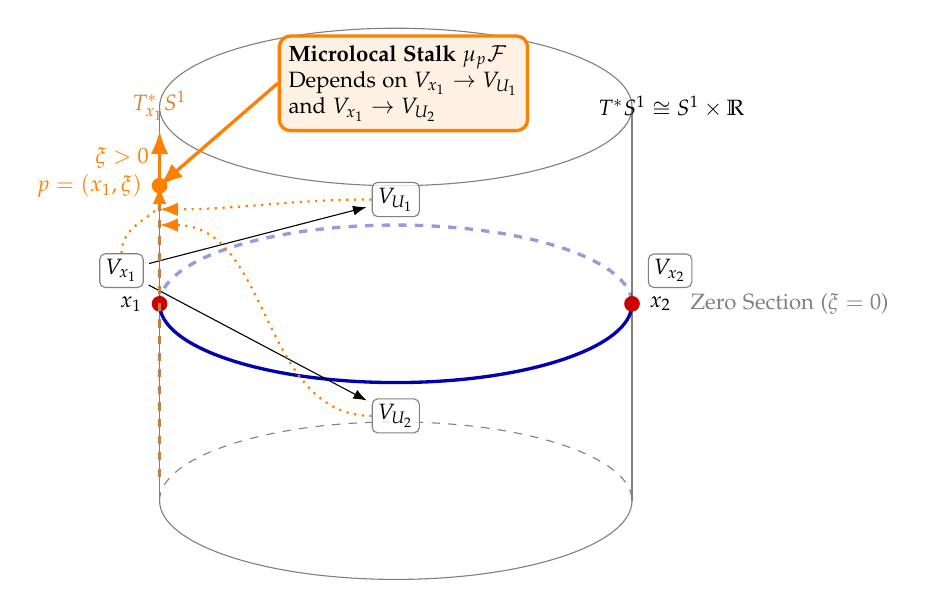
\begin{tikzpicture}[
    font=\footnotesize,
    >=Latex,
    % Define geometric parameters for the cylinder perspective
    x_rad/.style={x radius=3cm},
    y_rad_main/.style={y radius=1cm},
    y_rad_cap/.style={y radius=1cm},
    cylinder_height/.store in=\cylht, cylinder_height=2.5cm,
    % Define styles for strata and data
    stratum_point/.style={circle, fill=red!80!black, inner sep=2pt, outer sep=0pt},
    stratum_line/.style={very thick, blue!70!black},
    sheaf_data/.style={fill=white, fill opacity=0.8, text opacity=1, draw=gray, thin, rounded corners=2pt, inner sep=2pt},
    micro_point/.style={circle, fill=orange, inner sep=2pt},
    conormal_fiber/.style={thick, orange!50!gray, dashed}
]

% --- 1. Draw the Cylinder (Cotangent Bundle T*S^1) ---

% Bottom cap (back half dashed)
\draw[gray, dashed, x_rad, y_rad_cap] (-3,-\cylht) arc (180:0:3cm and 1cm);
\draw[gray, x_rad, y_rad_cap] (-3,-\cylht) arc (180:360:3cm and 1cm);

% Vertical walls
\draw[gray] (-3, -\cylht) -- (-3, \cylht);
\draw[gray] (3, -\cylht) -- (3, \cylht);

% Top cap
\draw[gray, x_rad, y_rad_cap] (0,\cylht) circle (3cm and 1cm);

% Label the spaces
\node at (3.5, \cylht) {$T^*S^1 \cong S^1 \times \mathbb{R}$};
\node[gray] at (5.0, 0) {Zero Section ($\xi=0$)};


% --- 2. Draw the Stratified Base Space S^1 (Zero Section) ---

% Define coordinates for the stratifying points
\coordinate (x1) at (-3, 0);
\coordinate (x2) at (3, 0);

% Interval U1 (Back semi-circle)
\draw[stratum_line, opacity=0.4, dashed, x_rad, y_rad_main] 
    (x1) arc (180:0:3cm and 1cm);
\coordinate (u1_mid) at (0, 0.9); % Midpoint for label

% Interval U2 (Front semi-circle)
\draw[stratum_line, x_rad, y_rad_main] 
    (x1) arc (180:360:3cm and 1cm);
\coordinate (u2_mid) at (0, -0.9); % Midpoint for label

% Points x1 and x2
\node[stratum_point, label={left:$x_1$}] at (x1) {};
\node[stratum_point, label={right:$x_2$}] at (x2) {};


% --- 3. Visualize Sheaf Data on the Base ---

% Stalks at points
\node[sheaf_data, anchor=south east] (Vx1) at ($(x1)+(-0.2,0.2)$) {$V_{x_1}$};
\node[sheaf_data, anchor=south west] (Vx2) at ($(x2)+(0.2,0.2)$) {$V_{x_2}$};

% Stalks on intervals
\node[sheaf_data, anchor=south] (Vu1) at ($(u1_mid)+(0,0.2)$) {$V_{U_1}$};
\node[sheaf_data, anchor=north] (Vu2) at ($(u2_mid)+(0,-0.3)$) {$V_{U_2}$};

% Draw restriction/generization maps (sp)
% From x1 to U1 and U2
\draw[->, shorten >=2pt, shorten <=2pt] (Vx1) -- (Vu1);
\draw[->, shorten >=2pt, shorten <=2pt] (Vx1) -- (Vu2);
% From x2 to U1 and U2 (optional, for completeness)
%\draw[->, shorten >=2pt, shorten <=2pt, opacity=0.5] (Vx2) -- (Vu1);
%\draw[->, shorten >=2pt, shorten <=2pt, opacity=0.5] (Vx2) -- (Vu2);


% --- 4. Visualize the Microlocal Stalk ---

% Draw the conormal fiber over x1 (T^*_{x1} S^1)
\draw[conormal_fiber] (-3, -2.2) -- (-3, 2.2) node[above, orange!70!gray] {$T^*_{x_1}S^1$};

% Pick a point p = (x1, xi) with xi > 0
\coordinate (p) at (-3, 1.5);
\node[micro_point] at (p) {};

% Add cotangent vector xi indicating direction
\draw[->, very thick, orange] (p) -- ++(0, 0.7) node[midway, left] {$\xi > 0$};
\node[left, orange] at ($(p)-(0.1,0)$) {$p=(x_1, \xi)$};

% Label the microlocal stalk
% We use a callout box to indicate it depends on local data
\node[draw=orange, very thick, fill=orange!10, rounded corners, align=left, anchor=west] 
    (micro_label) at (-1.5, 2.8) 
    {\textbf{Microlocal Stalk} $\mu_p\mathcal{F}$\\
     Depends on $V_{x_1} \to V_{U_1}$ \\
     and $V_{x_1} \to V_{U_2}$};

\draw[orange, very thick, ->] (micro_label.west) -- (p);

% Add visual connectors showing dependence
% Connecting the base data to the microlocal point to show the relationship
\draw[orange, dotted, thick, ->] (Vx1.north) to[out=90, in=270] (p);
\draw[orange, dotted, thick, ->] (Vu1.west) to[out=180, in=0] ($(p)+(0,-0.3)$);
\draw[orange, dotted, thick, ->] (Vu2.west) to[out=180, in=0] ($(p)+(0,-0.5)$);

\end{tikzpicture}
\end{center}
\caption{A microlocal stalk}%
\label{fig:microlocal_stalk}
\end{figure}


The following theorem inspired many subsequent works, including the lecturer's PhD work.
\begin{thm}[Nadler-Zaslow]
    The dg-category \(\ms{Sh}_c(X)\) of constructible sheaves on \(X\) equivalent the Fukaya category \(\ms{Fuk}(T^* X)\) of the cotangent bundle \(T^* X\) of \(X\).
\end{thm}
We will now discuss a geometric interpretation. We may consider the characteristic cycle \(\on{CC}(\mc{F})\) of a constructible sheaf, which is a conic Lagrangian cycle in \(T^* X\). However, the objects of the Fukaya category are smooth Lagrangian submanifolds with the cochain complexes of morphisms being given by counting interesection points and holomorphic polygons. See~\Cref{fig:fukaya} for a visualization. It is usually very difficult to calculate the Fukaya category directly, but the theorem allows us to translate these questions into questions about constructible sheaves, which are more manageable.
\begin{figure}[htpb]
\begin{center}
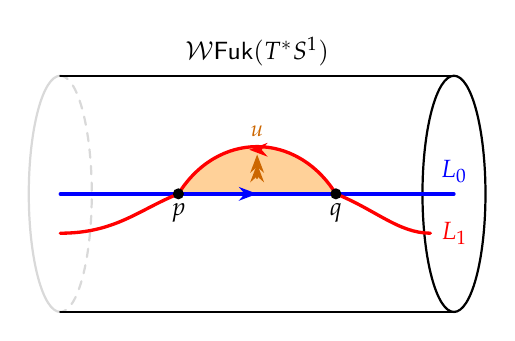
\begin{tikzpicture}[
    >=Stealth,
    font=\small,
    line cap=round,
    line join=round
]

% --- Definitions ---
\def\cylLen{6}   % Length of cylinder
\def\cylRad{1.5} % Radius of cylinder
\def\xStart{0.5}
\def\xEnd{5.5}

% --- Draw Back of Cylinder (Inside) ---
\draw[gray!30, thick] (\xStart, \cylRad) arc (90:270:0.4 and \cylRad);
\draw[gray!30, thick, dashed] (\xStart, \cylRad) arc (90:-90:0.4 and \cylRad);

% --- Draw Cylinder Body ---
% Top and Bottom lines
\draw[thick] (\xStart, \cylRad) -- (\xEnd, \cylRad);
\draw[thick] (\xStart, -\cylRad) -- (\xEnd, -\cylRad);

% Right Cap (Front)
\draw[thick] (\xEnd, 0) ellipse (0.4 and \cylRad);

% --- Define Lagrangians ---

% L0: The Zero Section (Straight horizontal line along the "front" face)
% We place it slightly offset in z-space conceptually, but y=0 in 2D
\coordinate (L0_start) at (\xStart, 0);
\coordinate (L0_end) at (\xEnd, 0);

% L1: An oscillating Lagrangian (e.g., graph of df or a wrapped curve)
% It creates a "Bigon" (two intersection points)
\coordinate (p) at (2, 0); % Intersection 1
\coordinate (q) at (4, 0); % Intersection 2

% --- Draw the Holomorphic Polygon (Shading) ---
% We fill the area between L0 and L1 between p and q
\fill[orange!90!yellow, opacity=0.4] 
    (p) 
    -- (2.2, 0) % Guide point along L0
    -- (q) 
    .. controls (3.5, 0.8) and (2.5, 0.8) .. (p);

% Add a flow arrow inside the polygon to indicate holomorphic map u
\draw[->, orange!80!black, thick, decoration={markings, mark=at position 0.6 with {\arrow{>}}}, postaction={decorate}] 
    (3, 0.2) -- (3, 0.5) node[above=0.1, font=\footnotesize] {$u$};

% --- Draw L0 (Blue) ---
\draw[blue, very thick] (L0_start) -- (L0_end) node[above] {$L_0$};

% --- Draw L1 (Red) ---
% Curve starts low, intersects p, goes high, intersects q, goes low
\draw[red, very thick] 
    (\xStart, -0.5) 
    .. controls (1.2, -0.5) and (1.5, -0.2) .. (p)
    .. controls (2.5, 0.8) and (3.5, 0.8) .. (q)
    .. controls (4.5, -0.2) and (4.8, -0.5) .. (5.2, -0.5)
    node[right] {$L_1$};

% --- Draw Intersection Points ---
\fill[black] (p) circle (2pt) node[below] {$p$};
\fill[black] (q) circle (2pt) node[below] {$q$};

% --- Annotations ---
\node[above] at (3, \cylRad) {$\mathcal{W}\ms{Fuk}(T^*S^1)$};

% Optional: Draw vector field or boundary orientation on the strip
% Top boundary orientation
\draw[->, red, thick] (3, 0.56) -- (2.9, 0.56); 
% Bottom boundary orientation
\draw[->, blue, thick] (2.9, 0) -- (3, 0);

\end{tikzpicture}
\end{center}
\caption{Two objects in the Fukaya category}%
\label{fig:fukaya}
\end{figure}


\begin{proof}[Sketch of proof]
    We will begin by discussing why there is a fully faithful functor \(\on{Sh}_c(X) \to \ms{Fuk}(T^* X)\). The first step is to find some nice generators of the constructible sheaf category. For this, we consider open embeddings \(j \colon U \hookrightarrow X\) and extension by zero \(j_! \C_U\) of the constant sheaf on \(U\). These have characteristic cycles given by the conormal bundle to the boundary \(\partial U\) (together with the zero section at \(U\)). We will send this sheaf \(j_! \C_U\) to a smoothing of its characteristic cycle, as depicted in~\Cref{fig:charcycle_smoothing}.
    \begin{figure}[htpb]
    \begin{center}
    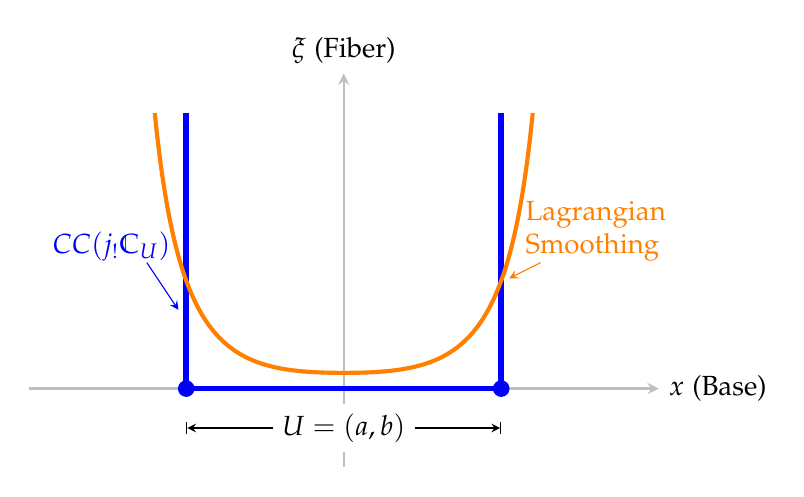
\begin{tikzpicture}[>=stealth, thick]

    % --- 1. Axes (T*R plane) ---
    \draw[->, gray!50] (-4, 0) -- (4, 0) node[right, black] {$x$ (Base)};
    \draw[->, gray!50] (0, -1) -- (0, 4) node[above, black] {$\xi$ (Fiber)};

    % Define Interval U = (-2, 2)
    \def\a{-2}
    \def\b{2}

    % --- 2. Singular Characteristic Cycle CC(F) ---
    % F = j_! C_U (Extension by zero)
    % Cycle = Zero section over U + Conormals at boundary
    % Drawn in BLUE
    
    % The Zero Section part: U x {0}
    \draw[blue, line width=2pt] (\a, 0) -- (\b, 0);
    
    % The Conormal parts: {a} x R+ and {b} x R+ (Upward orientation for visual standard)
    \draw[blue, line width=2pt] (\a, 0) -- (\a, 3.5);
    \draw[blue, line width=2pt] (\b, 0) -- (\b, 3.5);
    
    % Draw "Nodes" at the singularities (corners)
    \fill[blue] (\a, 0) circle (3pt);
    \fill[blue] (\b, 0) circle (3pt);


    % --- 3. Lagrangian Smoothing ---
    % A smooth approximation that rounds the corners
    % Drawn in ORANGE
    
    \draw[orange, line width=1.5pt] 
        (\a - 0.4, 3.5) 
        .. controls (\a - 0.1, 0.5) and (\a + 0.5, 0.2) .. (0, 0.2) % Left corner smoothing
        .. controls (\b - 0.5, 0.2) and (\b + 0.1, 0.5) .. (\b + 0.4, 3.5); % Right corner smoothing


    % --- 4. Annotations ---
    
    % Label the Interval U
    \draw[|<->|, thin, black] (\a, -0.5) -- (\b, -0.5) node[midway, fill=white] {$U = (a,b)$};
    
    % Label the Singular Cycle
    \node[blue, align=left] at (-2.95, 1.8) {$CC(j_! \mathbb{C}_U)$};
    \draw[->, blue, thin] (-2.5, 1.6) -- (-2.1, 1);
    
    % Label the Smoothing
    \node[orange, align=left] at (3.2, 2) {Lagrangian\\Smoothing};
    \draw[->, orange, thin] (2.5, 1.6) -- (2.1, 1.4);

\end{tikzpicture}
    \end{center}
    \caption{Characteristic cycle and its smoothing}%
    \label{fig:charcycle_smoothing}
    \end{figure}
    

    To prove essential surjectivity, all of the Hom complexes in the Fukaya category can be calculated using Morse theory. For more details, see the original paper by Nadler-Zaslow.
\end{proof}

One reason to consider the Fukaya category is homological mirror symmetry, which was originally proposed by Kontsevich. For certain symplectic manifolds \(M\), there is a \textit{mirror partner} \(\check{M}\), which is a complex algebraic variety, and Kontsevich conjectured that there is an equivalence of categories
\[ \ms{Fuk}(M) \simeq \ms{Coh}(\check{M}). \]
The simplest example is when \(M = T^* S^1\), where we need to consider the fully wrapped Fukaya category. We have an equivalence
\[ \mc{W}\ms{Fuk}(T^* S^1) \simeq \ms{Loc}(S^1) \]
(modulo technical details), but the upshot is that all characteristic cycles are supported inside the zero section. Local systems are on \(S^1\) are simply representations of \(\pi_1(S^1) \cong \Z\), which are simply modules over the group algebra \(\C[\Z] \cong \C[t, t^{-1}] = \mc{O}(\C^{\times})\). Ignoring finiteness conditions, these are simply quasicoherent sheaves on \(\C^{\times}\).

\begin{rmk}
    For the purposes of representation theory, we will treat \(\pi_1(S^1) = \mathbb{X}_{\bullet}(S^1)\) as cocharacters, which will be identified with the characters \(\mathbb{X}^{\bullet}(\C^{\times})\) on the mirror side. This picture generalizes if we consider algebraic tori of any rank and is a version of Langlands duality in the abelian case.
\end{rmk}

\begin{rmk}
    Homological mirror symemtry is closely related to the geometric Langlands correspondence, where we send the Hitchin system for \(G\) to the character variety for the Langlands dual group \(G^{\vee}\). There are some technical issues, but the Betti geometric Langlands correspondence is essentially homological mirror symmetry here.
\end{rmk}

One modification of this is to complexify the Fukaya side into \(T^* T\), and in this case the (appropriate version of the) wrapped Fukaya category  still reduces to local systems on \(T\). Traditionally, we considered \(T^* T_c\) (the cotangent bundle of the compact form) because of the SYZ mirror symmetry philosophy, which predicts that a manifold \(M\) and its mirror \(\check{M}\) have dual Lagrangian torus fibrations. In general, it is very hard to use SYZ to construct mirrors because there are usually singular fibers, which are hard to control.

However, one way to produce a mirror is to believe in homological mirror symmetry and then try to find a variety \(\check{M}\) such that
\[ \ms{Fuk}(M) \simeq \ms{Coh}(\check{M}). \]
If the fibration has a Lagrangian section, then each smooth fiber becomes a Lie group, so \(\ms{Fuk}(M)\) is expected to pick up a ``convolution'' symmetric monoidal structure, which should correspond to the tensor product of coherent sheaves in some kind of non-linear Fourier transform.

In the second part of the course, we will generalize the duality \(T^*T \leftrightarrow T^{\vee}\) to the universal centralizer (or Toda system) \(J_G\), where \(G\) is a semisimple complex Lie group. This is related to representation theory for two reasons.
\begin{itemize}
    \item \(J_G\) is also called the bi-Whittaker reduction and represents something like the generic part of the representation of \(G\), namely the ``commutative part'' of the Hecke category;
    \item If we add a loop to \(G\), then we obtain the affine Toda system;
    \item There is a partial (log) compactification \(\ol{J}_G^{\log}\) over the base \(\g^* \sslash G\) constucted by Balibanu whose fibers are a kind of regular Hessenberg variety (a generalization of Springer fibers). The central fiber is the Peterson variety \(Y_P\), which is a closed subvariety of the flag variety \(G/B\) and is related to the quantum cohomology of \(G^{\vee}/P^{\vee}\) via the isomorphism
    \[ QH^*(G^{\vee} / P^{\vee}) \cong \mc{O}(Y_P). \]
\end{itemize}

\part{Geometry of complex semisimple Lie algebras and groups}

\section{Review of semisimple Lie algebras/groups}%
\label{sec:Review of semisimple Lie algebras/groups}

Eventually, the groups we are interested in are \(\on{SL}_n(\C)\), \(\on{SO}_n(\C)\), and \(\on{Sp}_{2n}(\C)\) with Lie algebras \(\mf{sl}_n(\C)\), \(\so_n(\C)\), and \(\sp_{2n}(\C)\). However, along the way we will encounter groups like Borels and unipotent groups.

\subsection{Generalities}%
\label{sub:Generalities}


Every Lie group has both a left and right action of \(G\) on itself given by the multiplication map
\[ m \colon G \times G \to G. \]
We may consider the tangent space \(\g = T_e G\) at the identity, and left translation of vector fields gives an isomorphism
\[ L \colon G \times \g \xrightarrow{\sim} TG \qquad (g, \xi) \mapsto L_{g *} \xi. \]
The right action gives another trivialization
\[ R \colon G \times \g \xrightarrow{\sim} TG \qquad (g, \xi) \mapsto R_{g^{-1} *} \xi. \]
These two are related by the diagram
\begin{equation*}
\begin{tikzcd}
    G \times \g \ar{r}{L} \ar[swap]{d}{\iota \times (-1)} & TG \ar{d}{T\iota} \\
    G \times \g \ar{r}{R} & TG,
\end{tikzcd}
\end{equation*}
where \(\iota\) is the map sending an element of \(G\) to its inverse. If we fix \(\xi \in \g\), then applying \(L\) gives us a left-invariant vector field \(\xi^{\ell}\) on \(G\), and similarly applying \(R\) gives a right-invariant vector field \(\xi^r\). 

\begin{lem}\leavevmode
    \begin{enumerate}
        \item Left (resp.\ right) invariant vector fields on \(G\) are closed under the Lie bracket;
        \item The left and right-invariant vector fields induce the same Lie bracket on \(\g\).
    \end{enumerate}
\end{lem}

The main idea of the proof is that the Lie bracket is preserved by diffeomorphisms and in particular left (or right) translation. 

\begin{rmk}
    If we have any action \(a \colon G \times X \to X\), then taking the derivative
    \[ {(\d{a})_e} \colon \g \times X \to X \]
    gives an infinitesimal action of \(G\) on \(X\) (as in a map from \(\g\) to vector fields on \(X\)). For example, \(L\) is simply 
    \[ {(\d{m})_{e, \text{factor 2}}} \colon G \times \g \to TG \]
    and a similar statement is true for \(R\).
\end{rmk}

One important action of \(G\) on itself is the \textit{adjoint action}, where \(G\) acts on itself by conjugation. On the tangent space, we have \({(R_{g^{-1}})_*} L_{g*} = L_{g*} {(R_{g^{-1}})_*}\). By definition, we now have
\[ \Ad_g \xi \coloneqq {(R_{g^{-1}})_*} L_{g*} \xi, \]
which induces a map
\[ \Ad \colon G \to \GL(\g). \]
Therefore, another equivalent definition of the Lie bracket is to simply differentiate the adjoint action. There is also an exponential map \(\exp \colon \g \to G\), and the Lie bracket is defined as
\[ [\xi, \eta] \coloneqq \eval{\odv{}{t}}_{t=0} \Ad_{\exp(t\xi)} \eta. \]

\begin{rmk}
    Any finite-dimensional abstract Lie algebra is isomorphic to a subalgebra of \(\gl_n\) by Ado's theorem, which says that every finite-dimensional Lie algebra has a finite-dimensional faithful representation. In particular, every finite-dimensional Lie group over \(\R\) is locally an immersed subgroup of \(\GL_n(\R)\) for some \(n\).
\end{rmk}

We will give some principles of Lie theory:
\begin{itemize}
    \item The Lie group is (up to taking its universal cover) determined by its Lie algebra. Given a connected Lie group \((H, e)\), then any discrete covering \((H', e')\) inherits a unique group structure whose kernel lies in the center of \(H'\) (this works because the fundamental group of \(H\) is abelian due to the group structure). Conversely, any discrete central quotient of \(H\) is a Lie group with the same Lie algebra. If we work analytically, \(H\) has a universal cover, which is the unique simply connected Lie group with the same Lie algebra as \(H\).
    \item If \(G\) and \(H\) are Lie groups such that \(G\) is connected, then any Lie group homomorphism
    \[ \rho \colon G \to H \]
    is uniquely determined by its derivative \(\d{\rho} \colon \g \to \mf{h}\), which is a Lie algebra homomorphism.
    \item For \(\g = \on{\ms{Lie}} G\) and any embedding \(\mf{h} \hookrightarrow \g\), the subgroup of \(G\) generated by \(\exp(\mf{h})\) is an immersed Lie subgroup of \(G\) with Lie algebra \(\mf{h}\). For example, if \(G = S^1 \times S^1\) and \(\h\) is a line with irrational slope, then \(H\) is immersed rather than embedded.
    \item Let \(G\) and \(H\) be finite dimensional Lie groups with \(G\) connected and simply connected. Then a map \(f \colon T_e G \to T_e H\) is the differential of a Lie group homomorphism \(\rho \colon G \to H\) if and only if it is a Lie algebra homomorphism. The standard trick to prove this is to consider the graph
    \[ \g \hookrightarrow \g \oplus \h \qquad \xi \mapsto (\xi, f(\xi)), \]
    which is a Lie algebra embedding. Then we get an immersed subgroup of \(G \times H\) (this receives a map from \(G\) because \(G\) is simply connected), which we project down to \(H\).
\end{itemize}

By Ado's theorem, we see that the embedding \(\g \hookrightarrow \gl_n(\R)\) gives an immersed subgroup \(G \to \GL_n(\R)\). In addition, the third item actually implies that there is a unique simply connected Lie group for any Lie algebra \(\g\).

\begin{exm}
    Let \(X\) be a projective variety. Then studying the identity component \(\Aut(X)_{0}\) is similar to studying
    \[ T_e \Aut(X)_{0} = H^0(X, TX), \]
    which is a standard result in deformation theory. For example, if \(X = G/P\) is a partial flag variety, then \(H^0(X, TX) = \g\) in almost all cases, but if \(P=B\) (the full flag variety), then we really do have
    \[ H^0(X, TX) = \g. \]
    In particular, we have
    \[ \Aut(G/P)_{0} = G/Z(G), \]
    and when \(G\) is semisimple, the center is discrete.
\end{exm}

We will call a Lie algebra homomorphism
\[ \g \to \gl(V) \]
a \textit{representation} of \(\g\). For example, we previously considered the adjoint representation
\[ \ad \colon \g \to \gl(\g). \]
We can also take the direct sums \(V \oplus W\) and tensor products \(V \otimes W\) of representations.
It should be noted that the action on \(V \otimes W\) should take the form
\[ \xi (v \otimes w) = \xi v \otimes w + v \otimes \xi w \]
in analogy with differentiating the action of \(G\) on \(V \otimes W\), which takes the form
\[ g(v \otimes w) = gv \otimes gw. \]

\subsection{Rough classification of Lie algebras}%
\label{sub:Rough classification of Lie algebras}

Given a Lie algebra \(\g\), there is a \textit{lower central series}
\[ \g = D_0 \g \supset D_1(\g) = [\g,\g] \supset \cdots \supset D_{k-1}(\g) \supset D_k \g = [\g, D_{k-1} \g] \cdots \]
and the smaller \textit{derived series}
\[ \g = D^0\g \supset D^1 \g = [\g,\g] \supset \cdots \supset D^{k-1} \g \supset D^k \g = [D^{k-1}\g, D^{k-1}\g]. \]

\begin{defn}
    A Lie algebra is \textit{nilpotent} if the lower central series becomes zero at some point.
\end{defn}

One example of a nilpotent Lie algbera is if we consider upper-triangular matrices with zeroes on the diagonal (usually denoted \(\n\)).

\begin{defn}
    A Lie algebra is \textit{solvable} if the derived series eventually vanishes.
\end{defn}

An example of a solvable Lie algebra is the algebra \(\b\) of all upper-triangular matrices. The reason for this is that \([\b, \b] = \n\). If we write
\[ \b = \h \oplus \n, \]
then we see that \([\h, \h] = 0\), \([\h, \n] = \n\), and \([\n, \n] \subset \n\).

\begin{thm}[Engel]
    Let \(\g \subset \gl(V)\) be a Lie subalgebra such that every \(X \in \g\) is a nilpotent endomorphism of \(V\). Then there exists a nonzero \(v \in V\) such that \(X(v) = 0\) for all \(X \in \g\).
\end{thm}

Engel's theorem implies that all \(X \in \g\) can be made (strictly) upper-triangular simultaneously.

\begin{thm}[Lie]
    Let \(\g \subset \gl(V)\) be a solvable Lie subalgebra over \(\C\). Then there is a common eigenvector for all \(X \in \g\).
\end{thm}

In particular, Lie's theorem implies that all \(X \in \g\) can be simultaneously made upper-triangular.

We will now consider all solvable ideals in \(\g\). In fact, if we have a finite collection of solvable ideals, then the sum is still solvable, so there exists a maximal solvable ideal of \(\g\), called the \textit{radical} of \(\g\) and denoted \(\on{Rad}(\g)\). This fits into the exact sequence
\[ 0 \to \on{Rad}(\g) \to \g \to \g/\on{Rad}(\g) \to 0. \]


\subsection{Semisimple and reductive Lie algebras}%
\label{sub:Semisimple and reductive Lie algebras}

\begin{defn}
    A Lie algebra \(\g\) is \textit{semisimple} if \(\on{Rad}(\g) = 0\).
\end{defn}

\begin{exm}
    The Lie algebra \(\g / \on{Rad}(\g)\) is semisimple.
\end{exm}

\begin{defn}
    A Lie algebra is \textit{reductive} if \(\on{Rad}(\g) = Z(\g)\).
\end{defn}

\begin{rmk}
    There are other characterizations of reductive Lie algebras, for example that the nilradical (maximal nilpotent ideal) \(R_{\on{nil}}(\g)\), which fits into the exact sequence
    \[ 0 \to R_{\on{nil}}(\g) \to \g \to \g/R_{\on{nil}}(\g) \to 0, \]
    vanishes.
\end{rmk}

We now give some important properties of semisimple Lie algebras.
\begin{thm}
    Let \(\g\) be a semisimple Lie algebra. Then every finite-dimensional representation of \(\g\) decomposes uniquely as a direct sum of irreducible representations.
\end{thm}

\begin{proof}[Sketch of proof]
    There are two ways to do this, either algebraically (which is tedious) or by using Weyl's unitary trick. The key fact using the unitary trick is that every complex semisimple Lie algebra \(\g\) has a unique compact real form \(\g_c\) satisfying \(\g_c \otimes_{\R} \C = \g\) (being a real form) and being the Lie algebra of a simply connected compact Lie group.

    For example, the compact real form of \(\sl_n(\C)\) is \(\mf{su}_n\) (traceles anti-Hermitian matrices), which corresponds to \(\on{SU}_n \subset \on{SL}_n(\C)\). The unitary trick is to restrict to the action of the compact form \(G_c\) on \(V\) and then try to find a \(G_c\)-invariant Hermitian metric on \(V\), which will split \(W \subset V\) for free. The way to find the inner product is to pick any Hermitian metric \(\ab<-,->\) and a Haar measure \(\mu\) on \(G_c\) such that
    \[ \int_{G_c} \d{\mu} = 1, \] 
    and define a new inner product by
    \[ \ab<v,w>_{G_c} \coloneqq \int_{G_c} \ab<gv, gw> \d{\mu(g)} \]
    (which is the same trick we use for finite groups). Finally, the \(G_c\)-representations lift to \(G\), so we are done.
\end{proof}

\begin{thm}
    In fact, a Lie algebra is semisimple if and only if all of its finite-dimensional representations are semisimple.
\end{thm}

\begin{proof}
    Consider the adjoint representation \(\ad \colon \g \to \gl(\g)\). Because it is semisimple, we have a decomposition
    \[ \g = \on{Rad}(\g) \oplus \g/\on{Rad}(\g). \]
    In particular, we must have \([\on{Rad}(\g), \g_{\mr{ss}}] = 0\), where \(\g_{\mr{ss}} = \g / \on{Rad}(\g)\).

    If \(\on{Rad}(g) \neq 0\), then by Lie's theorem says that any representation must have an eigenvector, so all irreducible representations must be \(1\)-dimensional. This implies that
    \[ \g = \ell_1 \oplus \cdots \oplus \ell_k \oplus \g_{\on{ss}} = Z(\g) \oplus \g_{\mr{ss}}. \]
    Any abelian Lie algebra has indecomposable representations which are not semisimple, for example representing a line by matrices of the form \( \begin{bsmallmatrix}
        0 & * \\
        0 & 0
    \end{bsmallmatrix}    \), so the radical must have vanished to begin with.
\end{proof}

\begin{rmk}
    Levi's theorem actually states that \(\g = \on{Rad}(\g) \rtimes \g_{\mr{ss}}\).
\end{rmk}

\begin{thm}[Preservation of Jordan decomposition]
    Let \(\g\) be semisimple. For any \(X \in \g\), there exist \(X_s, X_n \in \g\) such that \(X_s + X_n = X\) and for any finite-dimensional representation
    \[ \rho \colon \g \to \gl(V), \]
    the Jordan normal form of \(\rho(X)\) has \({\rho(X)}_s = \rho(X_s)\) and \({\rho(X)}_n = \rho(X_n)\).
\end{thm}

\begin{rmk}
    If we consider the adjoint representation of \(\g\) (which is faithful), then in fact the condition on the Jordan decomposition in any representation actually implies that \(X = X_s + X_n\).
\end{rmk}

\begin{exm}
    If we consider \(\g = \C\), then the representation
    \[ t \mapsto \begin{bmatrix}
        t & t \\
        0 & t
    \end{bmatrix} \]
    has \({\rho(X)}_s\) and \({\rho(X)}_n\) not in the image of \(\rho\) in general.
\end{exm}

\begin{defn}
    If \(\g\) is semisimple, then we say \(X \in \g\) is \textit{semisimple} if \(X = X_s\) and \textit{nilpotent} if \(X = X_n\).
\end{defn}


We will now consider reductive Lie algebras. In fact, by Levi's theorem and the fact that \([Z(\g), \g_{\mr{ss}}] = 0\), \(\g\) is reductive if and only if it is the product of a semisimple and an abelian Lie algebra, which is equivalent to \(\g = Z(\g) \oplus [\g, \g]\).

\begin{defn}
    A Lie group is \textit{semisimple} if its Lie algebra is semisimple.
\end{defn}

We will now consider all complex semisimple Lie groups, which are actually affine algebraic groups. By Borel's theorem, they are actually all linear, meaning closed subgroups of some \(\GL_n\). If \(\g\) is semisimple, then there is a simply connected form \(G_{\on{sc}}\) and a tower down to the \textit{adjoint form} \(G_{\mr{sc}} = G_{\mr{sr}} / Z(G_{\mr{sc}})\).

\begin{exm}
    For the Lie algebra \(\sl_n\), then the simply connected form is \(\SL_n\) and the adjoint form is \(\on{PGL}_n\).
\end{exm}

\begin{exm}
    If we consider \(\sp_{2n}\), then the simply connected form is \(\Sp_{2n}(\C)\) and the adjoint form is \(\mr{P}\Sp_{2n}(\C)\).
\end{exm}

\begin{exm}
    For \(\SO_n\), there is a form \(\SO_n\), which for \(n \geq 3\) has fundamental group \(\Z/2\), so the simply connected form is the universal cover \(\on{Spin}_n\) and the adjoint form is \(\mr{P}\SO_n\).
\end{exm}

\begin{rmk}
    We may also consider simple Lie algebras, which are semisimple Lie algebras with no nontrivial ideals. Then the classical simple Lie algebras are the ones we have already listed and are the only infinite families.
\end{rmk}

There is also the Cartan-Killing criterion of semisimple Lie algebras.
\begin{defn}
    An \textit{invariant} bilinear form on \(\g\) is given by
    \[ B \colon \g \times \g \to \C \]
    satisfying the condition that 
    \[ \ad_x (B(y,z)) \coloneqq B([x,y], z) + B(y, [x,z]) = 0. \]
\end{defn}

\begin{defn}
    The \textit{Killing form} is the form
    \[ B(x,y) = \Tr (\ad_x \circ \ad_y). \]
    Because the trace has cyclic invariance and the trace is invariant under conjugation, this is invariant and symmetric.
\end{defn}

\begin{thm}[Cartan-Killing criterion]
    A Lie algebra \(\g\) is semisimple if and only if the Killing form is nondegenerate.
\end{thm}

In particular, the means that the adjoint and coadjoint representations are isomorphic.

\begin{rmk}
    If \(Z(\g) \neq 0\), then \(\ad_x = 0\) for all \(x \in Z(\g)\), so \(B(x, -) = 0\) for \(B\) the Killing form.
\end{rmk}


We now briefly pause to consider issues of analytic vs algebraic categories. If we are considering \textbf{semisimple} Lie groups over \(\C\), then they are in fact also (linear) algebraic groups. However, if we leave the semisimple setting, then there are differences. For example, if we consider \(\g = \C\), then the algebraic options are \((\C, +) = \G_a\), \((\C^{\times}, \times) = \G_m\), and compact \(1\)-dimensional tori, namely elliptic curves. Usually, in algebraic groups theory, we will only consider affine algebraic groups.

\begin{thm}[Borel]
    Every affine algebraic group \(G\) is linear, and has a closed immersion to some \(\GL(V)\).
\end{thm}


In the analytic world, there is the map
\[ \exp \colon \C \to \C^{\times}, \]
which is not algebraic. In particular, \(\G_a\) and \(\G_m\) are totally different and have no nontrivial morphisms between them (and we have to consider their formal completions to recover the exponential map). In fact, the category \(\ms{Rep}(\G_m)\) is semisimple (prove this using the unitary trick for \(S^1\)), while the same is not true for \(\G_a\) (consider the representation by matrices of the form \(\begin{bsmallmatrix}
    1 & * \\
    0 & 1
\end{bsmallmatrix}\)). However, any analytic Lie group over \(\C\) not containing a compact torus is algebraic.


We now proceed to defining reductive groups. Recall that we essentially need to figure out what to do with the center \(Z(\g)\) of a reductive Lie algebra \(\g\). In the algebraic group world, we will consider \textit{tori}, which are groups isomorphic to products of copies of \(\G_m\).

\begin{defn}
    A \textit{reductive} group \(G\) is a finite quotient of the product of an (affine) algebraic torus and a semisimple algebraic group.
\end{defn}

In particular, we have
\[ G = Z(G) \times^{Z(G^{\on{der}})} G^{\on{der}}, \]
where \(G^{\on{der}} = [G,G]\) is semisimple and \(Z(G)\) might be disconnected. For example, \(Z(\SL_n) = \mu_n\), which is clearly not connected. Alternatively, there is a quotient morphism
\[ G \to G / Z(G^{\on{der}}) = Z(G) / Z(G^{\on{der}}) \times G_{\ad}, \]
where again \(G_{\ad}= G/Z(G)\). Here, we see that \(Z(G)/Z(G^{\on{der}})\) is always connected. Using Langlands duality, we can produce a cover by something with connected center. A third alternative is to rewrite the product as
\[ G = Z(G)_0 \times^{Z{(G^{\on{der}})}^{0}} G^{\on{der}}, \]
where \(Z{(G^{\on{der}})}^{0} = Z(G)_0 \cap G^{\on{der}}\).

\begin{exm}
    In the case where \(G = \GL_n\), we have \(Z(\GL_n) = \C^{\times}\) and \({(\GL_n)}^{\on{der}} = \SL_n\), so we have
    \[ \GL_n = \C^{\times} \times^{\mu_n} \SL_n. \]
\end{exm}

Reductive \textbf{groups} are characterized by complete reducibility of their finite-dimensional representations (in characteristic zero). In addition, algebraic and analytic morphisms between reductive groups agree, so we no longer need to worry about the difference between algebraic and analytic categories. Representations of reductive groups also satisfy the preservation of Jordan decompositions, namely that for any \(g \in G\), there exist \(g_s, g_u \in G\) such that \(g = g_s g_u = g_u g_s\) and for any finite-dimensional representation
\[ \rho \colon G \to \GL(V), \]
the Jordan decomposition of \(\rho(g)\) satisfies \({\rho(g)}_s = \rho(g_s)\) and \({\rho(g)}_u = \rho(g_u)\).

\begin{lem}
    If \(\g\) is semisimple, then any invariant bilinear form is symmetric. In addition, any invariant non-degenerate bilinear form is a scalar multiple of the Killing form.
\end{lem}

\begin{proof}
    Any invariant bilinear form \(B\) induces a map
    \[ \g \to \g^* \]
    as morphisms of \(G \coloneqq G_{\ad}\)-representations. Recall that \(\g\) decomposes into a product 
    \[ \g = \g_1 \times \cdots \times \g_k \]
    of simple Lie algebras, so we have a morphism
    \[ \g_1 \times \cdots \times \g_k \to \g_1^* \times \cdots \times \g_k^*. \]
    Using the Killing form, we have an isomorphism \(\g_i \cong \g_i^*\), so by Schur's lemma, the map \(\g_i \to \g_j^*\) is zero if \(i \neq j\) and a scalar multiple of the identity if \(i = j\). Therefore, any invariant bilinear form is a sum of scalar multiples of Killing forms on each simple factor, which are all symmetric. The second statement follows similarly.
\end{proof}

\subsection{Cartan subalgebras}%
\label{sub:Cartan subalgebras}

We will begin by considering general \(\g\) and specialize to semisimple ones later. 

\begin{defn}
    If \(\mf{a} \subset \g\) is a Lie subalgebra, then the \textit{normalizer} of \(\mf{a}\) in \(\g\) is given by
    \[ \n_{\g}(\mf{a}) = \{ x \in \g : [x, \mf{a}] \subset \mf{a} \}. \]
\end{defn}

\begin{defn}
    A subalgebra \(\h \subset \g\) is a \textit{Cartan subalgebra} if 
    \begin{enumerate}
        \item \(\h\) is nilpotent;
        \item \(\h = \n_{\g}(\h)\) (as in it is equal to its own normalizer).
    \end{enumerate}
\end{defn}

We will see later that every Lie algebra has a Cartan subalgebra.

For any \(x \in \g\), let 
\[ P_x(T) = \det(T \on{Id} - \ad_x) = \sum_{i=0}^n a_i(x) T^i \] 
denote the characteristic polynomial of \(\ad_x\). If we choose linear coordinates \(x_1, \ldots, x_n\) on \(\g\), then each \(a_i(x)\) is a homogeneous polynomial in \(x_1, \ldots, x_n\) of degree \(n-i\). 

\begin{defn}
    The \textit{rank} of \(\g\) is the least \(i\) such that \(a_i(x)\) is not identically zero.
\end{defn}

\begin{exm}
    If \(\g \cong \C^n\) is abelian, then \(P_x(T) = T^n\) for all \(x\), so \(\g\) has rank \(n\).
\end{exm}

\begin{rmk}
    Note that \(i < n\) in the nonabelian case because \(a_n(x) = 1\) is never zero and \(i > 0\) because \(x \in \ker(\ad_x)\) for all \(x\) and therefore \(a_0(x) = 0\) for all \(x\).
\end{rmk}

From now on, we will denote the rank of \(\g\) by \(r\).

\begin{defn}
    We say that \(x \in \g \) is \textit{strongly regular} if \(a_r(x) \neq 0\).
\end{defn}

\begin{rmk}
    We will see another notion of regularity later, so we call this strongly regular to distinguish it.
\end{rmk}

We will denote the set of strongly regular elements by \(\g_{\on{sreg}}\). The definition of a strongly regular element implies the following.

\begin{prop}
    The set \(\g_{\on{sreg}}\) is a connected open dense subset of \(\g\) (in the Zariski topology and hence also the analytic topology).
\end{prop}

\begin{thm}
    If \(x \in \g_{\on{sreg}}\), then the generalized eigenspace of \(0\) for \(\ad_x\), denoted \(\g_x^0\), is a Cartan subalgebra of \(\g\).
\end{thm}

Note that by definition, we have \(\dim \g_x^0 = r\), so the dimension of this Cartan equals the rank of \(\g \). In fact, we have already described all Cartan subalgebras.

\begin{thm}
    Let \(\g\) be a Lie algebra over \(\C\). Then all Cartan subalgebras of \(\g\) are of the form \(\g_x^0\) for some \(x \in \g_{\on{sreg}}\).
\end{thm}

These Cartan subalgebras are all conjugate under the action of
\[ G_{\mr{inn}} = \ab<e^{\ad_x} \mid x \in \g> \hookrightarrow \Aut(\g), \]
so in particular \(G_{\mr{inn}}\) acts transitively on the set of Cartan subalgebras.

\begin{rmk}
    If \(G\) is reductive, then \(G_{\mr{inn}} = G_{\on{ad}} = G/Z(G)\).
\end{rmk}

\subsection{Root systems}%
\label{sub:Root systems}

We will now specialize to the semisimple case, which is much more explicit. 

\begin{thm}
    Let \(\h\) be a Cartan subalgebra of a semisimple Lie algebra \(\g\). Then
    \begin{enumerate}
        \item \(\h\) is abelian;
        \item \(\h\) is its own centralizer, i.e. \(Z_{\g}(\h) = \h\);
        \item Every element of \(\h\) is semisimple.
        \item The restriction of the Killing form to \(\h\) is nondegenerate.
    \end{enumerate}
\end{thm}

\begin{exm}
    If \(\g = \sl_n\), then the Cartan subalgebras are precisely the conjugates of the diagonal matrices. This has dimension \(n-1\) (given the constraint that the trace vanishes), so the rank of \(\sl_n\) is \(n-1\).
\end{exm}

For a semisimple Lie algebra, if \(x \in \h = \g_x^0\), then in fact \(\h = \ker \ad_x\) for a general choice of \(x\). The necessary condition on \(x\) is that it is \textit{regular semisimple}, which we can take to simply mean that \(\ker \ad_x\) is as small as possible. Because we can simultaneously diagonalize all \(\ad_x\) for \(x \in \h\), we have a decomposition
\[ \g = \h \oplus \bigoplus_{\alpha \in \Phi} \g_{\alpha}, \]
where
\[ \g_{\alpha} = \{ x \in \g : [h,x] = \alpha(h) x \text{ for all } h \in \h \} \]
and \(\Phi\) is the set of nonzero \(\alpha \in \h^*\) such that \(\g_{\alpha} \neq 0\). 

\begin{exm}
    Returning to \(\sl_n\), if we let
    \[ \h = \ab\{ \bdiagmat{x_1, \ddots, x_n} \}, \]
    then twe see that 
    \[ \ab[\bdiagmat{x_1, \ddots, x_n}, E_{ij}] = (x_i - x_j) E_{ij}. \]
    If we refer to the coordinates on \(\C^n\) as \(e_1, \ldots, e_n\), then the roots are given by
    \[ \Phi = \ab\{ \alpha_{ij} = e_i^* - e_j^* \mid i \neq j \}, \]
    where \(\alpha_{ij}(\bdiagmat{x_1, \ldots, x_n}) = x_i - x_j\). We refer to the set \(\Phi\) as the \textit{roots} of \(\g\) with respect to \(\h\) and \(\g_{\alpha}\) as the \textit{root space} corresponding to \(\alpha\).
\end{exm}

Because the Killing form is nondegenerate when restricted to \(\h\), we may identify \(e_i^* - e_j^* \in \h^*\) with \(e_i - e_j \in \h\). In particular, we may consider \(\Phi\) as a subset of \(\h\) itself.

\begin{cor}\leavevmode
    \begin{enumerate}
        \item \(\h\) is a maximal abelian subalgebra of \(\g\);
        \item Every strongly regular element is semisimple;
        \item \(G_{\ad}\) acts transitively on the set of all Cartan subalgebras of \(\g\). 
    \end{enumerate}
\end{cor}

\begin{warn}
    Not all maximal abelian subalgebras are Cartan subalgebras, for example the nilpotent matrices in \(\sl_2\).
\end{warn}

\begin{lem}
    Assume that \(G\) is semisimple. Let \(T = N_G(\h)_0\) (usually, it is not connected). Then \(T\) is a maximal torus in \(G\) with \(T \cong {(\C^{\times})}^r\).
\end{lem}

\begin{proof}[Sketch of proof]
    Choose a compact real form \(\g_c \subset \g\). We now consider the set
    \[ \g_{\mr{sreg}} \cap \g_c \neq \emptyset. \]
    Now let \(\xi_c \in \g_c\) be strongly regular. Then \(Z_{\g_c}(\xi_c) = \h_c\) is a Cartan subalgebra of \(\g_c\). Next, the normalizer
    \[ N_{G_c}{(\h_c)}_0 = Z_{G_c}{(\xi_c)}_0 = T_c \]
    is a maximal torus of \(G_c\) of real dimension \(r\), so we can conclude the proof by complexifying everything.
\end{proof}

\begin{exm}
    In the case of \(\sl_n\), if \(\xi\) is strongly regular, then we see that \(a_r(\xi) \neq 0\), and so \(\dim \ker \ad_{\xi} = r = n-1\), so \(\xi\) must be semisimple. In particular, the root space decomposition is
    \[ \g = \h \oplus \bigoplus_{i \neq j} \g_{\alpha_{ij}}. \]
\end{exm}

\begin{lem}
    Choose a root decomposition
    \[ \g = \h \oplus \bigoplus_{\alpha \in \Phi} \g_{\alpha}. \]
    Then \(\xi \in \h\) is strongly regular if and only if there exists \(\alpha \in \Phi\) such that \(\alpha(\xi) \neq 0\) for all \(\alpha \in \Phi\).
\end{lem}

\begin{proof}
    Note that \(\xi \in \h\) is strongly regular if and only if \(\ker \ad_{\xi} = \h\), which holds if and only if \(\ad_{\xi}|_{\g_{\alpha}}\) is nonzero for all \(\alpha \in \Phi\), which holds if and only if \(\alpha(\xi) \neq 0\) for all \(\alpha \in \Phi\).
\end{proof}

\begin{rmk}
    From now on, we will refer to strongly regular elements as \textit{regular semisimple} elements in the semisimple case and refer to the set of such elements as $\g_{\mr{rs}}$. We will also denote
    \[ \h^{\on{reg}} \coloneqq \g_{\mr{rs}} \cap \h, \]
    which is given by the equation
    \[ \prod_{\alpha \in \Phi} \alpha \neq 0. \]
\end{rmk}

\begin{exm}
    The Lie algebra \(\g = \sl_2\) is generated by the matrices
    \[ e = \begin{bmatrix}
        0 & 1 \\
        0 & 0
    \end{bmatrix}, \qquad f = \begin{bmatrix}
        0 & 0 \\
        1 & 0
    \end{bmatrix}, \qquad \text{and} \qquad h = \begin{bmatrix}
        1 & 0 \\
        0 & -1
    \end{bmatrix}, \]
    with the relations
    \[ [h,e] = 2e, \qquad [h,f] = -2f, \qquad \text{and} \qquad [e,f] = h. \]
    Then we see that the Cartan is \(\h = \C h\) and the root spaces are \(\g_{\alpha} = \C e\) and \(\g_{-\alpha} = \C f\), where \(\alpha(h) = 2\). Therefore, the root system is \(\Phi = \{\alpha, -\alpha\}\) and is shown in~\Cref{fig:sl2-roots}. In this case, a choice of \(\alpha\) is the same as choosing a set \(\Phi^+ \subset \Phi \) of positive roots. In this case, \(\alpha\) is also a simple root, but in general positive and simple roots are not the same.

    \begin{figure}[htpb]
    \begin{center}
    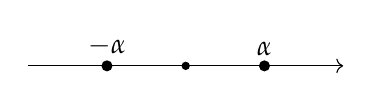
\begin{tikzpicture}[scale=1, transform shape]
          \draw[->] (-2,0) -- (2,0);
  \fill (1,0) circle (2pt) node[above] {$\alpha$};
  \fill (-1,0) circle (2pt) node[above] {$-\alpha$};
  \fill (0,0) circle (1.5pt);
    \end{tikzpicture}
    \end{center}
    \caption{Root system of \(\sl_2\)}%
    \label{fig:sl2-roots}
    \end{figure}

    Now set $\alpha^{\vee} = h \in \h$, which is a \textit{simple coroot}. Then we have $\ab<\alpha^{\vee}, \alpha> = 2$. We may now consider the maximal torus
    \[ \SL_2 \supset T = e^{2 \pi i s h} = \ab\{ \bdiagmat[empty={}]{t,t^{-1}} \} \cong \C / \Z h, \]
    The adjoint action of \(T\) on \(\g\) is given by
    \begin{align*}
        \Ad \ab(\bdiagmat[empty={}]{t,t^{-1}}) e &= \bdiagmat[empty={}]{t,t^{-1}} \begin{bmatrix}
            0 & 1 \\
            0 & 0
        \end{bmatrix} \bdiagmat[empty={}]{t^{-1},t} \\
        &= \begin{bmatrix}
            0 & t \\
            0 & 0
        \end{bmatrix} \bdiagmat[empty={}]{t^{-1},t} \\
        &= \begin{bmatrix}
            0 & t^2 \\
            0 & 0
        \end{bmatrix}.
    \end{align*}
    Note that \(\alpha (h) = 2\), which matches the exponent. We may now consider the \textit{cocharacter lattice}
    \begin{align*}
        \X_{\bullet}(T) &= \Hom(\C^{\times}, T) \\
        &\cong \pi_1 (T) \\
        & \cong \Z h \\
        &= \Z \alpha^{\vee}.
    \end{align*}
    If we project down to the adjoint form \(\on{PGL}_2 = \SL_2 / \pm I\) we see in fact that
    \[ \X_{\bullet} (T_{\ad}) = \Z \cdot \ab(\frac{1}{2} h). \]
    Note that this cocharacter lattice is dual to the root lattice and is called the \textit{coweight lattice}. We can now identify the \textit{character lattice} of \(T = T_{\on{sc}}\) with the \textit{weight lattice} $\Z \cdot \frac{1}{2} \alpha$, whereas $\X^{\bullet}(T_{\ad}) = \Z \cdot \alpha$ is the root lattice.
\end{exm}

Now consider the exact sequence
\[ 1 \to Z(G_{\on{sc}}) \to G_{\on{sc}} \to G_{\ad} \to 1. \]
This induces the exact sequence
\[ 1 \to \pi_1(G_{\on{sc}}) \to \pi_1(G_{\ad}) \to Z(G_{\on{sc}}) \to 1. \]
In particular, we see once again that $\pi_1(G_{\ad}) \cong Z(G_{\on{sc}})$. If we instead consider maximal tori, we have
\[ 1 \to Z(G_{\on{sc}}) \to T_{\on{sc}} \to T_{\ad} \to 1, \]
which induces the exact sequence
\[ 0 \to \X_{\bullet}(T_{\on{sc}}) \to \X_{\bullet}(T_{\ad}) \to Z(G_{\on{sc}}) \to 0 \]
on fundamental groups. This gives us the identification
\[ \pi_1(G_{\ad}) \cong \X_{\bullet}(T_{\ad}) \cong Z(G_{\on{sc}}) \cong \X_{\bullet}(T_{\ad}) / \X_{\bullet}(T_{\on{sc}}) \]
and relates the coroot and coweight lattices.

\begin{exm}
    In the case of $\sl_3$, the root system is drawn in~\Cref{fig:sl3-roots}. In particular, the roots are given by
    \[ \Phi = \ab\{ \alpha_{ij} \colon \alpha_{ij} \ab(\diagmat[empty={}]{x_1, x_2, x_3}) = x_i - x_j \middle\vert i \neq j \}. \]

    \begin{figure}[htpb]
    \begin{center}
         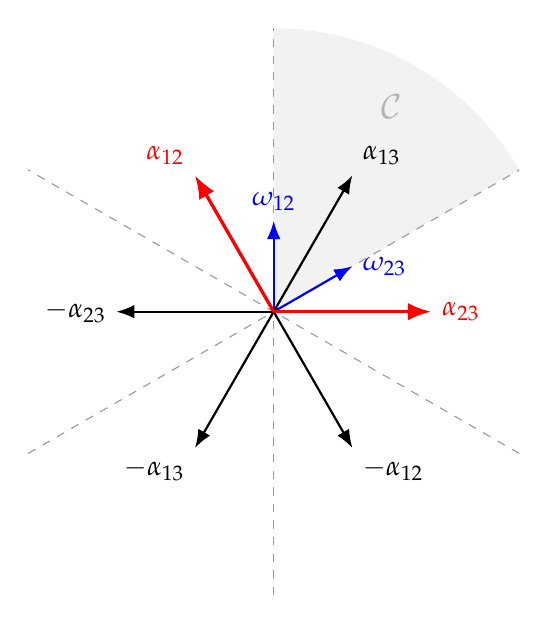
\begin{tikzpicture}[scale=2, >=Latex]

    % -------------------------------------------------------
    % 1. Shade the Fundamental Weyl Chamber
    % -------------------------------------------------------
    % The chamber is the cone defined by <v, alpha_i> >= 0.
    % It is bounded by the hyperplanes orthogonal to the simple roots.
    % H_alpha1 is at 90 degrees. H_alpha2 is at 30 degrees.
    \fill[gray!10] (0,0) -- (30:1.8) arc (30:90:1.8) -- cycle;
    \node[gray!60, font=\large] at (60:1.5) {$\mathcal{C}$};

    % -------------------------------------------------------
    % 2. Draw Hyperplanes (orthogonal to roots)
    % -------------------------------------------------------
    % These extend infinitely (or to the edge of our view)
    \foreach \angle in {30, 90, 150} {        \draw[dashed, gray!80] (\angle:-1.8) -- (\angle:1.8);
    }

    % -------------------------------------------------------
    % 3. Draw Fundamental Weights
    % -------------------------------------------------------
    % omega1 is dual to alpha1 check. It lies on the boundary H_alpha2 (30 deg).
    % omega2 lies on the boundary H_alpha1 (90 deg).
    % Length: If roots have length 1, weights have length 1/sqrt(3) approx 0.577
    \def\wlen{0.577}
    \draw[->, blue, thick] (0,0) -- (30:\wlen) node[right] {$\omega_{23}$};
    \draw[->, blue, thick] (0,0) -- (90:\wlen) node[above] {$\omega_{12}$};

    % -------------------------------------------------------
    % 4. Draw Roots
    % -------------------------------------------------------
    \def\rlen{1.0} % Root length

    % Non-simple positive root
    \draw[->, thick] (0,0) -- (60:\rlen) node[above right] {$\alpha_{13}$};

    % Negative roots
    \draw[->, thick] (0,0) -- (180:\rlen) node[left] {$-\alpha_{23}$};
    \draw[->, thick] (0,0) -- (240:\rlen) node[below left] {$-\alpha_{13}$};
    \draw[->, thick] (0,0) -- (300:\rlen) node[below right] {$-\alpha_{12}$};

    % Simple Roots (Highlighted)
    \draw[->, very thick, red] (0,0) -- (0:\rlen) node[right] {$\alpha_{23}$};
    \draw[->, very thick, red] (0,0) -- (120:\rlen) node[above left] {$\alpha_{12}$};
\end{tikzpicture}
    \end{center}
    \caption{Root system of \(\sl_3\)}%
    \label{fig:sl3-roots}
    \end{figure}

    In order to treat the coroots, note that
    \[ \sl_2 \cong \g_{\alpha} \oplus \g_{-\alpha} \oplus [\g_{\alpha}, \g_{-\alpha}] \]
    for any root \(\alpha\). Therefore, we may choose \(e_{\alpha} \in \g_{\alpha}\) and \(f_{\alpha} \in \g_{-\alpha}\) such that
    \[ [e_{\alpha}, f_{\alpha}] = h_{\alpha} \in \h. \]
    For example, if we consider \(\alpha = \alpha_{12}\), then we may choose
    \[ e_{\alpha} = \begin{bmatrix}
        0 & 1 & 0 \\
        0 & 0 & 0 \\
        0 & 0 & 0
    \end{bmatrix}, \qquad f_{\alpha} = \begin{bmatrix}
        0 & 0 & 0 \\
        1 & 0 & 0 \\
        0 & 0 & 0
    \end{bmatrix}, \qquad h_{\alpha} = \bdiagmat[empty={}]{1,-1,0}. \]
    We now have the coroot \(\alpha_{ij}^{\vee} = h_{\alpha_{ij}}\) such that 
    \( \ab<\alpha_{ij}^{\vee}, \alpha_{ij}> = 2 \). 

    To choose a basis, we cut \(\h^*\) by a general linear hyperplane and choose a positive direction. This gives a set $\Phi^+$ of positive roots. For example, we will choose \(\Phi^+ = \ab\{ \alpha_{ij} \mid i < j\}\) for \(\sl_3\). Inside this, there is a \textbf{unique} set of simple roots \(\Pi \subset \Phi^+\) satisfying
    \begin{enumerate}
        \item It is a basis of \(\h_{\R}\);
        \item Any \(\beta \in \Phi^+\) is a nonnegative integer combination of elements of \(\Pi\).
    \end{enumerate}
    For example, in this case, we have \(\Pi = \{\alpha_{12}, \alpha_{23}\} \subset \Phi^+ \). The simple coroots are then simply \(\Pi^{\vee} = \ab\{ \alpha_{12}^{\vee}, \alpha_{23}^{\vee} \} \).
    Then the \textit{Cartan matrix} is given by
    \[ C \coloneqq \begin{bmatrix}
        \ab<\alpha_{12}^{\vee}, \alpha_{12}> & \ab<\alpha_{12}^{\vee}, \alpha_{23}> \\[4pt]
        \ab<\alpha_{23}^{\vee}, \alpha_{12}> & \ab<\alpha_{23}^{\vee}, \alpha_{23}>
    \end{bmatrix} = \begin{bmatrix}
        2 & -1 \\
        -1 & 2
    \end{bmatrix}. \]

    We should also explain why the picture has the angles as shown. If we recall that the root lattice \(Q\) is identified with the character lattice \(X^{\bullet}(T_{\ad})\), this is proved by considering the kernel \(\ker Q \subset T_{\ad}\). In particular, anything killed by \(Q\) must actually act trivially on the root spaces and acts trivially on \(\h\) by definition, so it lives in the center of \(G_{\ad}\), which is trivial. Continuing as before, we consider the coweight lattice, which is spanned by the matrices
    \[ \omega_{i+1,i+2}^{\vee} \coloneqq\frac{1}{3} (\ep_i + \ep_{i+1} - 2 \ep_{i+2}), \qquad \ep_i = E_{ii}. \]

    \begin{figure}[htpb]
    \begin{center}
         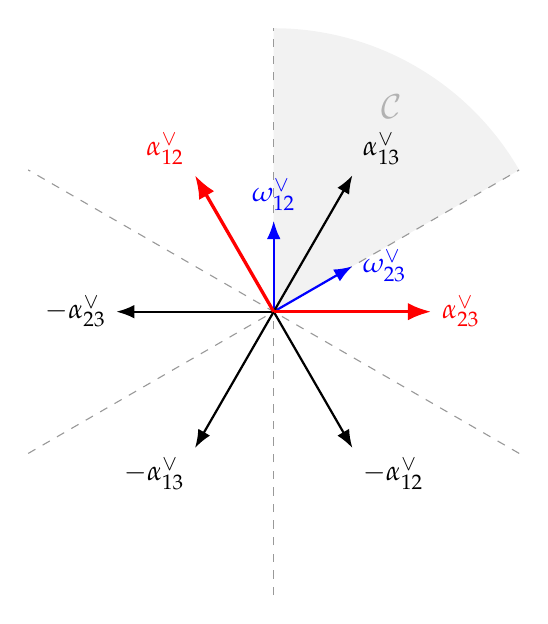
\begin{tikzpicture}[scale=2, >=Latex]

    % -------------------------------------------------------
    % 1. Shade the Fundamental Weyl Chamber
    % -------------------------------------------------------
    \fill[gray!10] (0,0) -- (30:1.8) arc (30:90:1.8) -- cycle;
    \node[gray!60, font=\large] at (60:1.5) {$\mathcal{C}$};

    % -------------------------------------------------------
    % 2. Draw Hyperplanes (orthogonal to coroots)
    % -------------------------------------------------------
    \foreach \angle in {30, 90, 150} {
      \draw[dashed, gray!80] (\angle:-1.8) -- (\angle:1.8);
    }

    % -------------------------------------------------------
    % 3. Draw Fundamental Coweights (optional)
    % -------------------------------------------------------
    \def\wlen{0.577}
    \draw[->, blue, thick] (0,0) -- (30:\wlen) node[right] {$\omega_{23}^{\vee}$};
    \draw[->, blue, thick] (0,0) -- (90:\wlen) node[above] {$\omega_{12}^{\vee}$};

    % -------------------------------------------------------
    % 4. Draw Coroots
    % -------------------------------------------------------
    \def\rlen{1.0}

    % Non-simple positive coroot
    \draw[->, thick] (0,0) -- (60:\rlen) node[above right] {$\alpha_{13}^{\vee}$};

    % Negative coroots
    \draw[->, thick] (0,0) -- (180:\rlen) node[left] {$-\alpha_{23}^{\vee}$};
    \draw[->, thick] (0,0) -- (240:\rlen) node[below left] {$-\alpha_{13}^{\vee}$};
    \draw[->, thick] (0,0) -- (300:\rlen) node[below right] {$-\alpha_{12}^{\vee}$};

    % Simple coroots (Highlighted)
    \draw[->, very thick, red] (0,0) -- (0:\rlen) node[right] {$\alpha_{23}^{\vee}$};
    \draw[->, very thick, red] (0,0) -- (120:\rlen) node[above left] {$\alpha_{12}^{\vee}$};
    \end{tikzpicture}
    \end{center}
    \caption{Coroot system of \(\sl_3\)}%
    \label{fig:sl3-coroots}
    \end{figure}
\end{exm}

\begin{rmk}
    The Cartan matrix is symmetric if and only if the Dynkin diagram is simply laced, i.e. has no multiple edges.
\end{rmk}

Unfortunately, we will not be able to discuss root systems in detail for time reasons. In type A (where \(\g = \sl_{n+1}\)), the picture generalizes that of \(\sl_3\), where we can choose \(\Phi^+ = \ab\{ \alpha_{ij} \mid i < j\}\) and \(\Pi = \ab\{\alpha_{i,i+1} \mid 1 \leq i \leq n\}\). As a remark, we will also refer to the weight lattice as \(P\) and the coweight lattice as \(P^{\vee}\). In general, we will interpret the fundamental weights \(\omega_i\) as the dual basis to the simple coroots \(\alpha_i^{\vee}\).

In the group picture, if we have an intermediate form \(G\) with maximal torus \(T\), then we have the inclusions
\[ \X_{\bullet}(T_{\on{sc}}) \subset \X_{\bullet}(T) \subset \X_{\bullet}(T_{\ad}) \]
induced by
\[ T_{\on{sc}} \to T \to T_{\ad}. \]
To find the center of \(G\), we simply have the quotient \(Z(G) = X_{\bullet}(T_{\ad}) / X_{\bullet}(T) \), which comes from the long exact sequence on homotopy groups coming from 
\[ 1 \to Z(G) \to T \to T_{\on{ad}} \to 1. \]
To find the fundamental group of \(G\), we apply this to the exact sequence
\[ 1 \to \pi_1(G) \to T_{\on{sc}} \to T \to 1, \]
which gives us \(\pi_1(G) = X_{\bullet}(T) / X_{\bullet}(T_{\on{sc}})\). In particular, this specializes to
\[ \X_{\bullet}(T_{\ad}) / \X_{\bullet}(T_{\on{sc}}) = Z(G_{\on{sc}}) = \pi_1(G_{\ad}). \]
For example, if \(G_{\on{sc}} = \SL_3\), then we have
\[ Z(G_{\on{sc}}) = \X_{\bullet}(T_{\ad}) / \X_{\bullet}(T_{\on{sc}}) \cong \Z / 3 \Z. \]
Because this group has prime order, there are no intermediate forms between \(\SL_3\) and \(\on{PGL}_3\).

Using the Killing form, there is the formula
\begin{align*}
    \ab<\alpha^{\vee}, \beta> &= \frac{2 (\alpha, \beta)}{(\alpha, \alpha)} \\
    &= \frac{2 \norm{\alpha} \norm{\beta} \cos\theta}{\norm{\alpha}^2} \\
    &= 2 \frac{\norm{\beta}}{\norm{\alpha}} \cos\theta,
\end{align*}
and this actually implies that
\begin{align*}
    \ab<\alpha^{\vee}, \beta> \ab<\beta^{\vee}, \alpha> &= 2 \frac{\norm{\alpha}}{\norm{\beta}} \cos\theta \cdot 2 \frac{\norm{\beta}}{\norm{\alpha}} \cos\theta \\
    &=  4 \cos^2 \theta.
\end{align*}
Because this needs to be an integer, we see that for all roots, the angle \(\theta\) between them must satisfy \(4 \cos^2 \theta \in \Z \). This restricts the possible angles to \(\frac{\pi}{2}, \frac{2\pi}{3}, \frac{\pi}{3}, \frac{\pi}{4}, \frac{3\pi}{4}, \frac{\pi}{6}\), or \(\frac{5\pi}{6}\) unless \(\alpha = \pm \beta\).

\begin{rmk}
    Root systems are classified by \textit{Dynkin diagrams}, which is equivalent to classifying Cartan matrices. The entries of the Cartan matrix satisfy \(C_{ii} = 2\) and \(C_{ij} \leq 0\). Non-symmetry can be explained by the fact that in some root systems, \(\alpha_i\) and \(\alpha_j\) may have different lengths. This gives arise to the notions of \textit{long roots} and \textit{short roots}. In fact, there are only two possible lengths for all roots (under the Weyl group action, any root can become simple).
\end{rmk}

For an example of a root system with two lengths, consider the \(B_2\) root system, whose root and coroot systems are shown in~\Cref{fig:b2-roots-coroots}.

\begin{figure}[htpb!]
    \begin{subfigure}{0.4\textwidth}
        \begin{center}
            \scalebox{0.6}{
            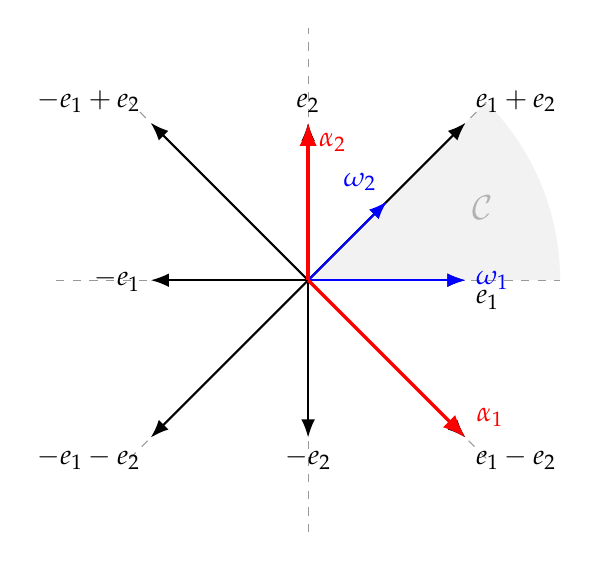
\begin{tikzpicture}[scale=2, >=Latex]

% -------------------------------------------------------
% 1. Shade the Fundamental Weyl Chamber
% -------------------------------------------------------
% Chamber: <v,alpha2>=y>=0 and <v,alpha1>=x-y>=0 (i.e. 0 <= angle <= 45)
\fill[gray!10] (0,0) -- (0:1.6) arc (0:45:1.6) -- cycle;
\node[gray!60, font=\large] at (22.5:1.2) {$\mathcal{C}$};

% -------------------------------------------------------
% 2. Draw Hyperplanes (orthogonal to roots)
% -------------------------------------------------------
% Orthogonal to e2 (0 deg), e1 (90 deg), e1-e2 (45 deg), e1+e2 (135 deg)
\foreach \angle in {0,45,90,135} {
  \draw[dashed, gray!80] (\angle:-1.6) -- (\angle:1.6);
}

% -------------------------------------------------------
% 3. Draw Fundamental Weights
% -------------------------------------------------------
% omega1 = e1, omega2 = (e1+e2)/2
\def\short{1}
\def\wone{1}


% -------------------------------------------------------
% 4. Draw Roots
% -------------------------------------------------------

% Short roots: ±e1, ±e2
\draw[->, thick] (0,0) -- (0:{\short}) node[below right] {$e_1$};
\draw[->, thick] (0,0) -- (180:{\short}) node[left] {$-e_1$};
\draw[->, thick] (0,0) -- (90:{\short}) node[above] {$e_2$};
\draw[->, thick] (0,0) -- (270:{\short}) node[below] {$-e_2$};

% Long roots: ±(e1+e2), ±(e1-e2)
\draw[->, thick] (0,0) -- (45:{sqrt(2)}) node[above right] {$e_1+e_2$};
\draw[->, thick] (0,0) -- (225:{sqrt(2)}) node[below left] {$-e_1-e_2$};
\draw[->, thick] (0,0) -- (315:{sqrt(2)}) node[below right] {$e_1-e_2$};
\draw[->, thick] (0,0) -- (135:{sqrt(2)}) node[above left] {$-e_1+e_2$};

\draw[->, blue, thick] (0,0) -- (0:1) node[right] {$\omega_1$};
\draw[->, blue, thick] (0,0) -- (45:{sqrt(2)/2}) node[above left] {$\omega_2$};

% Simple roots (Highlighted)
\draw[->, very thick, red] (0,0) -- (315:{sqrt(2)}) node[above right] {$\alpha_1$};
\draw[->, very thick, red] (0,0) -- (90:1) node[below right] {$\alpha_2$};

\end{tikzpicture}}
        \end{center}
        \caption{Root system of \(B_2\)}
        \label{fig:b2-roots}
    \end{subfigure}
    \begin{subfigure}{0.5\textwidth}
        \begin{center}
            \scalebox{0.6}{
            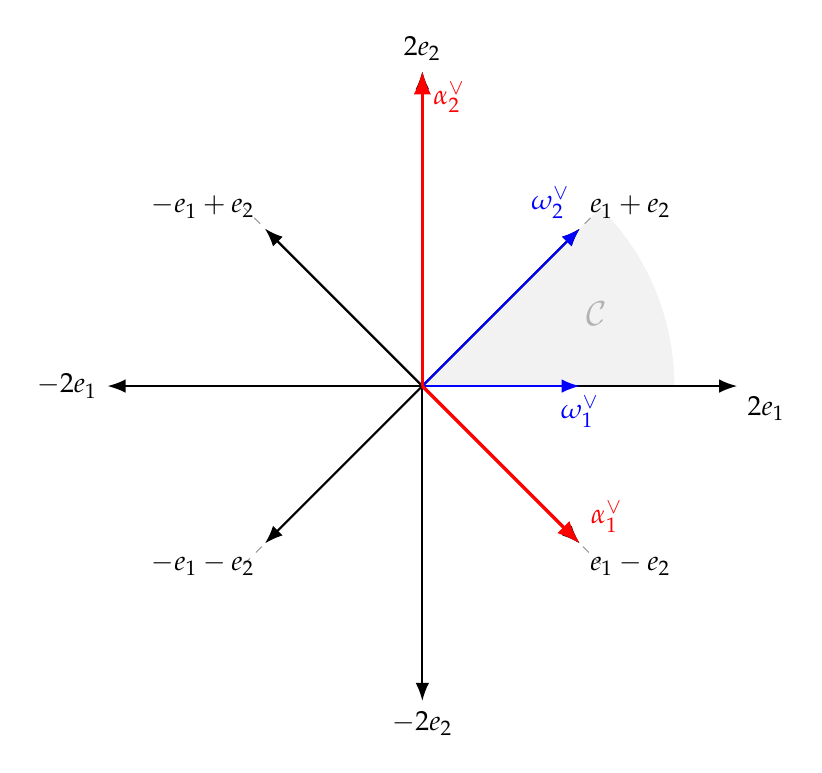
\begin{tikzpicture}[scale=2, >=Latex]

% -------------------------------------------------------
% 1. Shade the Fundamental Weyl Chamber
% -------------------------------------------------------
% Same chamber: 0 <= angle <= 45
\fill[gray!10] (0,0) -- (0:1.6) arc (0:45:1.6) -- cycle;
\node[gray!60, font=\large] at (22.5:1.2) {$\mathcal{C}$};

% -------------------------------------------------------
% 2. Draw Hyperplanes (orthogonal to coroots)
% -------------------------------------------------------
\foreach \angle in {0,45,90,135} {
  \draw[dashed, gray!80] (\angle:-1.6) -- (\angle:1.6);
}

% -------------------------------------------------------
% 3. Draw Fundamental Coweights
% -------------------------------------------------------
% omega1^vee = e1, omega2^vee = e1+e2
\def\wone{1}
\def\wtwo{sqrt(2)}

% -------------------------------------------------------
% 4. Draw Coroots
% -------------------------------------------------------
% short coroots: ±(e1±e2), long coroots: ±2e1, ±2e2
\def\short{sqrt(2)}

% Long coroots: ±2e1, ±2e2
\draw[->, thick] (0,0) -- (0:2) node[below right] {$2e_1$};
\draw[->, thick] (0,0) -- (180:2) node[left] {$-2e_1$};
\draw[->, thick] (0,0) -- (90:2) node[above] {$2e_2$};
\draw[->, thick] (0,0) -- (270:2) node[below] {$-2e_2$};

% Short coroots: ±(e1+e2), ±(e1-e2)
\draw[->, thick] (0,0) -- (45:{\short}) node[above right] {$e_1+e_2$};
\draw[->, thick] (0,0) -- (225:{\short}) node[below left] {$-e_1-e_2$};
\draw[->, thick] (0,0) -- (315:{\short}) node[below right] {$e_1-e_2$};
\draw[->, thick] (0,0) -- (135:{\short}) node[above left] {$-e_1+e_2$};

\draw[->, blue, thick] (0,0) -- (0:{\wone}) node[below] {$\omega_1^{\vee}$};
\draw[->, blue, thick] (0,0) -- (45:{\wtwo}) node[above left] {$\omega_2^{\vee}$};


% Simple coroots (Highlighted)
\draw[->, very thick, red] (0,0) -- (315:{\short}) node[above right] {$\alpha_1^{\vee}$};
\draw[->, very thick, red] (0,0) -- (90:2) node[below right] {$\alpha_2^{\vee}$};

\end{tikzpicture}}
        \end{center}
        \caption{Coroot system of \(B_2\)}
        \label{fig:b2-coroots}
    \end{subfigure}
    \caption{Root and coroot systems of type \(B_2\)}%
    \label{fig:b2-root-coroot}
\end{figure}


\subsection{Weyl groups}%
\label{sub:Weyl groups}

Recall that the maximal torus \(T\) has Lie algebra \(\h\). Then we define the \textit{Weyl group}
\[ W_T \coloneqq N_G(T) / T. \]
Here, we know that \(\n_{\g}(\h) = \h\), so \(T \subset N_G(T)\).

\begin{exm}
    If \(g = \sl_n\), then \(W_T \cong S_n\) because we can permute the diagonal entries.
\end{exm}

The Weyl group acts on the set \(\Phi\) of roots. Each root \(\alpha\) corresponds to a reflection \(s_{\alpha} \in W_T\) given by
\begin{align*}
    s_{\alpha}(x) &= x - \ab<\alpha^{\vee}, x>\alpha \\
    &= x - \frac{2 (\alpha, x)}{(\alpha, \alpha)} \alpha.
\end{align*}
This satisfies \(s_{\alpha}^2 = \mr{id}\) and fixes the hyperplane \(\alpha^{\perp} \subset \h^*\) pointwise. 

In the \(\sl_n\) example, the root \(\alpha_{ij}\) corresponds to the reflection that swaps the \(i\)-th and \(j\)-th coordinates. In particular, its kernel is the set of all matrices satisfying \(x_i = x_j\).

The Weyl group is generated by the \textit{simple reflections}, which correspond to the simple roots \(\Pi\). We will refer to the simple roots as \(\alpha_i \in \Pi\) and the corresponding reflections as \(s_i = s_{\alpha_i}\). Then, the Weyl group has the presentation
\[ W_T = \ab<s_i \mid s_i^2 = e, \ldots >. \]
and is a finite \textit{reflection group}.

The reflection hyperplanes \(\alpha^{\perp}\) cut the space \(\h^*_{\R}\) into a set of chambers, which are fundamental domains for the Weyl action and are in bijection with the choices of positive roots \(\Phi^+\). 
In particular, the set \(\Phi^+\) corresponds to the chamber
\begin{align*}
    C_{\Phi^+} &= \ab\{ \mu \in \h^*_{\R} \mid \ab<\alpha^{\vee}, \mu> \geq 0 \text{ for all } \alpha^{\vee} \in \Phi^{\vee, +} \} \\
    &= \ab\{ \mu \in \h_{\R} \mid \ab<\alpha^{\vee}, \mu> \geq 0 \text{ for all } \alpha^{\vee} \in \Pi^{\vee, +} \} \\
    &= \on{Span}_{\R_{\geq 0}} \ab\{ \omega_i \mid 1 \leq i \leq r \}.
\end{align*}
Note also that the choice of a set of positive roots corresponds to a choice of Borel \(\b \supset \h\). In particular, there is the direct sum decomposition
\[ \b = \h \oplus \bigoplus_{\alpha \in \Phi^+} \g_{\alpha}. \]
In addition, for any \(\alpha, \beta \in \Phi\) we have
\[ [g_{\alpha}, g_{\beta}] = \begin{cases}
    g_{\alpha + \beta} & \alpha + \beta \in \Phi, \\
    \k \alpha^{\vee} & \alpha + \beta = 0, \\
    0 & \text{otherwise}.
\end{cases} \]






\part{Universal centralizers}





\end{document}

%%% Local Variables:
%%% mode: latex
%%% TeX-master: t
%%% End:
